\chapter{Kognitivismus}
\label{cha:Kognitivismus}
%Nachdem die beiden Abschnitte \ref{sub:Kopiermodell} und \ref{sub:LernenDurchAnregung} grundlegende Darstellungen der allgemeinen didaktischen Aufbereitung von Wissen mit Hilfe zweier Modelle gezeigt hat, beschreibt dieses Kapitel die Lerntheorie des Kognitivismus.%

%\section{Definition}\label{Definition Kognitivismus} %FB Keine Zwischenüberschrift nötig.
Diese in den Sechzigerjahren des letzten Jahrhunderts entwickelte Theorie beschreibt anders als die bis dahin vorherrschende behavioristische Lerntheorie, auf welche aufgrund des beschränkten Umfangs dieser Arbeit nicht eingegangen werden kann, nicht ausschließlich das Ergebnis des Lernprozesses, sondern die bis dahin als 'Black Box' verstandene Verarbeitung sowie Strukturierung von Wissen im Gehirn des Menschen. \cite[S. 155]{Erpenbeck.2007} 
Weiter kann der Kognitivismus als die Theorie beschrieben werden, welche die \textbf{Wahrnehmungs-}, \textbf{Denk-}, \textbf{Verstehens-}, sowie \textbf{Denkprozesse} näher betrachtet. Hierbei wird der Mensch als Informationsverarbeitungseinheit angesehen. Er funktioniert ähnlich wie das aus der elektronischen Datenverarbeitung bekannte Datenverarbeitungsprinzip \textbf{EVA} (Eingabe, Verarbeitung, Ausgabe), wobei der Forschungsfokus dieser Theorie auf der Verarbeitung liegt. Folgende Abbildung verdeutlicht diese zusätzlich. \cite{AnsgarA.PlassmannProf.Dr.GunterSchmitt.2007}

\begin{figure}[h]
	\centering
	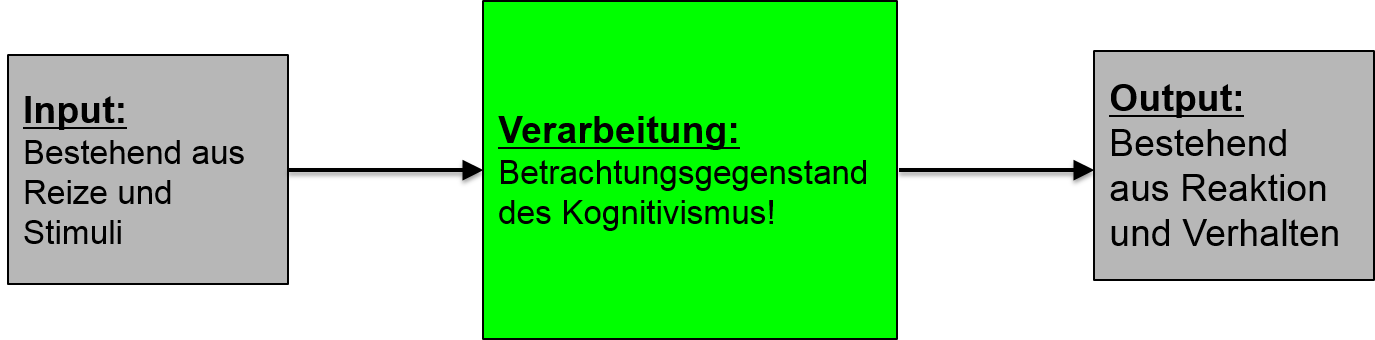
\includegraphics[width=1.0\textwidth]{Abbildungen/Kognitivismus1.PNG}
	\caption{Kognitivismus als EVA-Darstellung. In Anlehnung an \cite[S. 12]{SusanneMeir.}}
	\label{fig:Kognitivismusdarstellung}
\end{figure}

\section{Lernregeln des Kognitivismus sowie die Anwendung im E-Learning}
Folgende fünf kognitivistischen Lernregeln sollten nach \cite{Vontobel.2006} bei der Wissensvermittlung grundsätzlich, egal welche Lerntheorie bzw. didaktisches Modell (vgl. \ref{sec:Lernmodelle}) berücksichtigt wird, beachtet werden. Diese Lernregeln fokussieren sich nicht ausschließlich, jedoch hauptsächlich auf die in der Einleitung von Kapitel \ref{cha:Kognitivismus} erwähnte Datenverarbeitungsprozesse im Gehirn des Menschen, weshalb auf diese im Rahmen dieser Lerntheorie eingegangen wird.\cite[S. 10]{Vontobel.2006}

Vontobel beschreibt als erste Lernregel, das \textbf{Wecken der Aufmerksamkeit} des Lernenden. Ohne grundsätzliche Aufmerksamkeit (Vigilanz) ist kein Lernprozess möglich, sodass keine Wissenvermittlung stattfinden kann. Zur Einhaltung dieser Lernregel kann die Nutzung von Filmen, Animationen, sowie die Formulierung von Lernzielen erfolgen. Wichtig hierbei ist die Vermeidung von Monotonie. \cite[S. 10f.]{Vontobel.2006} %Vigilanz entweder sprachlich erläutern/erklären warum der Begriff genannt wird, oder rauslassen

Als zweite Lernregel wird die \textbf{Aktivierung von Vorwissen} beschrieben. Für die effiziente Überführung von Wissen im Kurzzeit- hin zum Langzeitgedächtnis hat sich die Verknüpfung von neuem mit bestehendem Wissen bewährt. Vontobel empfiehlt hierfür das Aufzeigen der Quintessenz des neu zu Erlernenden bereits zu Beginn der Wissensvermittlung. Das Anwenden von Vorwissenstests (Multiple Choice, Stellungnahme zu einer formulierten Fragestellung usw.) unterstützt durch grafische Darstellungen sowie die Erläuterung in wie weit neuer Lernstoff mit Altem in Verbindung steht, unterstützt die Umsetzung. \cite[S. 11f.]{Vontobel.2006} %Zwei Sätze aus letztem Satz machen

Die \textbf{Unterstützung des Wahrnehmungsprozesses}, dem Erkennen eines Reizes (bspw. eine gezeigte Information in Form eines Videos), fördert die effiziente Einordnung der Information im Gehirn. Hierbei soll auf die angemessene Gestaltung der Lerninhalte geachtet werden. Es empfiehlt sich eine Darstellung welche die Bildschirmgröße nicht überschreitet. Dies vermeidet das Scrollen und portioniert die Information optimal. Hierfür kann im E-Learning-Kontext die gezielte Abgrenzung mit Hilfe von Weißräumen, die Aufteilung der Inhalte auf mehrere Darstellungsseiten (Screens), sowie die abwechselnde Nutzung diverser Medien (Text, Bild, Ton usw.) verwendet werden.\cite[S. 12f.]{Vontobel.2006} %Erster Satz: DEM?; Bildschirmgröße kommt unvermittelt. Allgemeinerer Ausdruck: Grenzen des Lehrmediums? oder E-Learning früher erwähnen

Eine weitere Lernregel beschreibt die \textbf{Verbesserung der Speicherung von Wissen im Gedächtnis}. Dies wird durch die Kombination der vorhergegangen Lernregeln erreicht. Hierbei stellt die Bildung eines 'Superzeichens' eine weitere Methodik dar. Dieses auch unter dem Begriff 'Eselsbrücke' bekannte Schema soll als Lernanker dienen, welcher es dem Lernenden erlaubt Wissen langfristig abzuspeichern und schnell abzurufen. \cite[S.14]{Vontobel.2006}   
        
Die \textbf{Lernkontrolle} ist die letzte zu nennende Lernregel. \cite[S. 15]{Vontobel.2006} Sie ist für den Lernprozess wichtig um weiteren Lernbedarf zu identifizieren. Hierbei können eine Reihe von Werkzeugen genutzt werden. Selbsttests, Multiple-Choice-Fragen sowie Lückentexte eignen sich besonders gut für die automatisierte Wissensüberprüfung. Darüber hinaus fördern Sie das Selbstvertrauen des Lernenden und geben ihm neben der Lernzielformulierung einen Schwerpunktüberblick über das gerade Erlernte. \cite[S. 72f.]{Drummer.2011} Weitere Instrumente können dem Buch 'E-Learning im Unterricht' entnommen werden (siehe \cite{Drummer.2011}).   %den abschließenden Verweis würde ich weglassen, da ja das Buch bereits einige male vorher erwähnt wird.


